\section{VLBI}\label{sec:vlbi}
To achieve larger and larger resolution in astronomical imaging, it is
necessary to build larger telescopes, or to revert to
interferometry. As interferometry combines the measurements of several
telescopes to simulate a dish of a size equivalent to the maximal
distance between the farthest telescopes on the plane orthogonal to
the viewing direction. Numerous arrays (groups of telescopes) use this
technique, e.g., the VLA (Very Large Array), Lofar (Low-frequency
array), the EVN (European VLBI Network) or the VLBA (Very Large
Baseline Array).  Interferometry with telescopes that are
geographically very far apart is refered to as Very Large Baseline
Interferometry (VLBI). With VLBI it is possible to build a virtual
radio-telescope with a dish of size of the Earth. As the angular
resolution of a VLBI experiment depends on the maximal projected
distance between two radio-telescopes, VLBI achieves unsurpassed
angular resolution with the drawback of a relatively low sensitivity
\cite{VLBIbook}\marginpar{NGHK: TODO}. Another important property is
sensitivity, as it allows to detect fainter astronomical
objects. Increasing the sensitivity is possible by adding more
radio-telescopes or by increasing the sampling rate or
resolution. Increasing the sampling rate or resolution increases the
data rate per telescope.

In order to get the final picture the signal gathered from the
radio-telescopes have to be correlated at a central place, the Joint
Institute for VLBI in Europe (JIVE).  JIVE is
operating a dedicated hardware correlator~\cite{EVNCorrelator}.

The maximal capacity of this hardware correlator is 16 telescopes at a
data rate of 1Gbs each. The requirements on both the data streams and
the computing power are shown in Table~\ref{tab:speed}.

% \marginpar{NGHK: Check 16Mb/s in table}
\begin{table}
  \centering
  \begin{tabular}[c]{|l|l|l|l|l|l|}
    \hline
    Description & \# & \#  & data-rate & spect/prod & Tflops\\
    & telescopes & sub-bands & (Mb/s) &  & \\
    \hline
    \hline
    Fabric-demo &4 &2 &16 &32 &0.16\\
    1 Gb/s, full array  &16 &16 &1024 &16 &83.39\\
    future VLBI &32 &32 &4096 &256 &\verb|~|21457\\
    \hline
  \end{tabular}
  \caption{Network bandwidths and computing power needed for an {\it e}-VLBI
    experiment based on a XF architecture.}
  \label{tab:speed}
\end{table}

\begin{figure}
  \centering 
  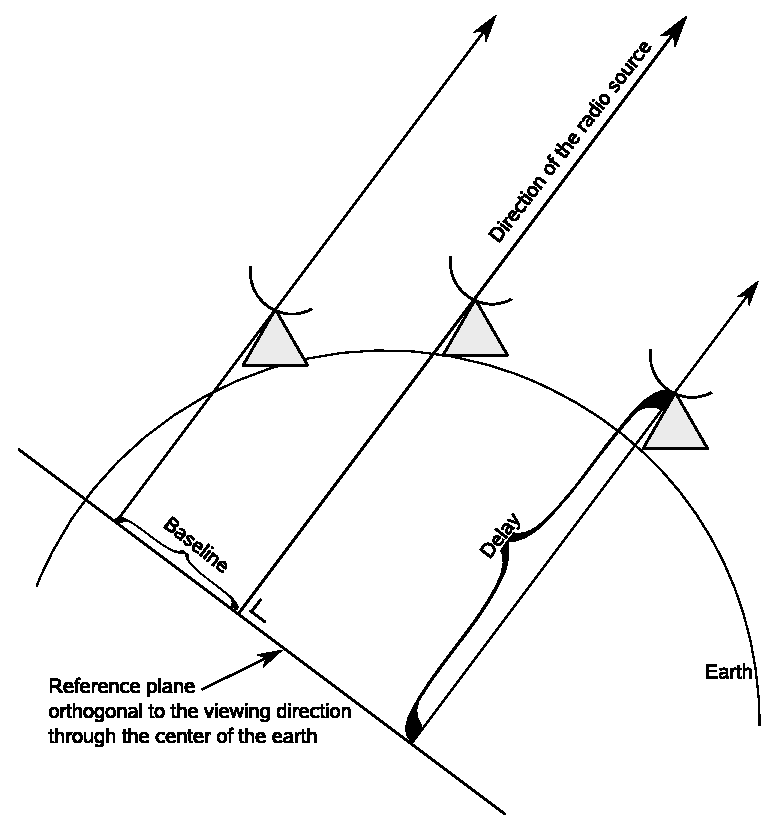
\includegraphics[width=0.5\textwidth]{img/VLBI.eps}
  \caption{Aligning the signals before correlation.}
  \label{fig:correlation_diagram}
\end{figure}

\paragraph{{\it e}-VLBI}
Traditionally, in VLBI, the data is recorded at the telescopes on disk
packs during an experiment. After the experiment the disks are shipped
to a central institute. There can be several weeks between the
experiment and the time when the correlated data becomes available.

Currently, JIVE is in the transition phase from traditional VLBI to
{\it e}-VLBI~\cite{szomoru-2004}. In an electronic VLBI ({\it e}-VLBI)
experiment, data from the telescopes is transferred directly over the
internet to JIVE, where it is streamed into the correlator in real
time. The data transport from the telescopes to JIVE goes over several
networks like local connections, paths provided by NRENs and the
G\'EANT backbone in Europe.

Transporting the data over the network has several advantages over a
traditional experiment. Obviously, the results of the experiments are
almost immediately available. This opens up the possibility to change
the course of an experiment based on earlier findings. Also, {\it
  e}-VLBI allows for real time analysis of the data and helps to
identify and resolve minor technical problems in the data collection
during the experiment.

Several experiments in the past have shown that real time {\it e}-VLBI
is possible. The EC funds the EXPReS project%
%\footnote{EXPReS is made
%  possible through the support of the European Commission (DG-INFSO),
%  Sixth Framework Programme, Contract \#026642.}
~\cite{EXPReS} which aims at building a production-level {\it e}-VLBI
instrument of upto 16 intercontinental telescopes connected in
real-time to JIVE and available to the general astronomy community.

\paragraph{Correlation}
Correlation is the process by which data from multiple telescopes is
collected and combined to measure the spatial Fourier components of
the image of the sky. It consists of two steps: first applying a delay
correction to align the signals and secondly computing the correlation
function for each pair of telescopes called a baseline.

To align the signals from the different telescopes, we project all the
telescopes on the plane through the center of the earth and orthogonal
to direction to the source, see
Figure~\ref{fig:correlation_diagram}. We will correlate the signals
received by the virtual projected telescopes. To compute these
signals, the signals from the real telescopes are delayed with the
distance between the telescope and its projection multiplied with the
speed of light (the signal travels with the speed of light). Note that
the delay changes during the observation because the earth rotates. We
conveniently split the delay in an integer number of samples and a
remaining fraction. While the integer delay is easily done by an
offset in the sample buffer, the fractional bit shift is usually
implemented as a phase rotation in the frequency domain. In a final
step, called the phase rotation, we change the sample rate to match
the rate of the delay function.

After the delay has been applied, the signals are ready for
correlation. Correlation~\cite{def_correlation} is mathematically
defined as a function on two signals in which the first signal is
delayed with discrete steps and the integral is computed of the
delayed signal multiplied with the second signal. The correlation is
done for each baseline (pair of telescopes). The correlation is called
an auto-correlation if the signal of a station is correlated with
itself and a cross-correlation if the signals are from different
stations. Note that the complexity of the correlation is quadratic in
the number of telescopes, as it is linear in the number of baselines.

To increase the signal to noise ratio, the correlated signal is
averaged over a certain period of time. Typical averaging times lie in
the range of $0.25-4$ seconds. Finally, the averaged signals are
Fourier transformed. Correlation in this order is refered to as XF,
because the correlation is done before the Fourier transform.  This is
how the correlation is implemented in most hardware correlators, as it
allows for large parallelisation.

One of the properties of correlation is that the Fourier transform of
two correlated signals is equal to multiplying the Fourier transformed
signals~\cite{corr_theorem}. This relation is used in most software
correlators, where correlation is more expensive than multiplication.
After the delay, the signal from each telescope is Fourier transformed
and the signals for each baseline are then multiplied elementwise.
This implementation is also refered to as FX: the Fourier transform comes
before the correlation.

%%% Local Variables:
%%% mode: latex
%%% TeX-master: "Ingrid"
%%% End:
